\section{eo\-Parser Class Reference}
\label{classeo_parser}\index{eoParser@{eoParser}}
eo\-Parser: command line parser and configuration file reader This class is persistent, so it can be stored and reloaded to restore parameter settings.  


{\tt \#include $<$eo\-Parser.h$>$}

Inheritance diagram for eo\-Parser::\begin{figure}[H]
\begin{center}
\leavevmode
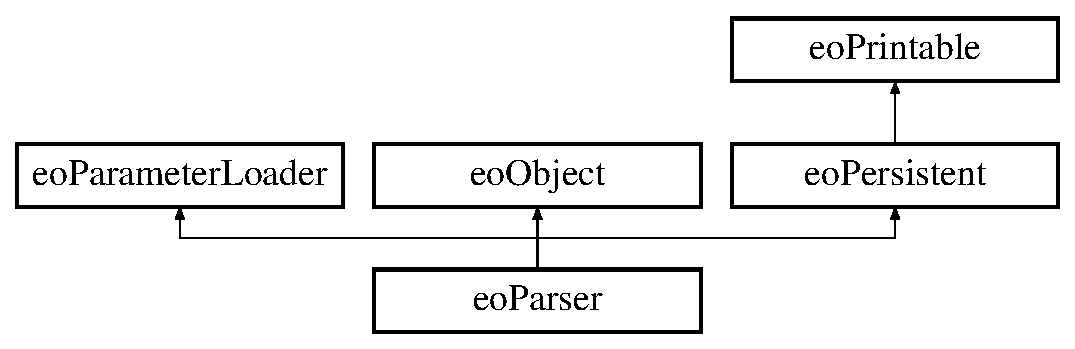
\includegraphics[height=3cm]{classeo_parser}
\end{center}
\end{figure}
\subsection*{Public Member Functions}
\begin{CompactItemize}
\item 
{\bf eo\-Parser} (unsigned \_\-argc, char $\ast$$\ast$\_\-argv, std::string \_\-program\-Description=\char`\"{}\char`\"{}, std::string \_\-l\-File\-Param\-Name=\char`\"{}param-file\char`\"{}, char \_\-short\-Hand= 'p')
\begin{CompactList}\small\item\em Constructor a complete constructor that reads the command line an optionally reads a configuration file. \item\end{CompactList}\item 
void {\bf process\-Param} ({\bf eo\-Param} \&param, std::string section=\char`\"{}\char`\"{})\label{classeo_parser_a1}

\begin{CompactList}\small\item\em Processes the parameter and puts it in the appropriate section for readability. \item\end{CompactList}\item 
void {\bf read\-From} (std::istream \&is)
\begin{CompactList}\small\item\em Read object. \item\end{CompactList}\item 
void {\bf print\-On} (std::ostream \&os) const 
\begin{CompactList}\small\item\em Write object. \item\end{CompactList}\item 
std::string {\bf class\-Name} (void) const \label{classeo_parser_a4}

\begin{CompactList}\small\item\em class\-Name for readibility \item\end{CompactList}\item 
bool {\bf user\-Needs\-Help} (void)\label{classeo_parser_a5}

\begin{CompactList}\small\item\em true if the user made an error or asked for help \item\end{CompactList}\item 
void {\bf print\-Help} (std::ostream \&os)\label{classeo_parser_a6}

\begin{CompactList}\small\item\em Prints an automatic help in the specified output using the information provided by parameters. \item\end{CompactList}\item 
std::string {\bf Program\-Name} ()\label{classeo_parser_a7}

\item 
virtual bool {\bf is\-It\-There} ({\bf eo\-Param} \&\_\-param) const 
\begin{CompactList}\small\item\em Has param been entered by user? \item\end{CompactList}\item 
{\bf eo\-Param} $\ast$ {\bf get\-Param\-With\-Long\-Name} (const std::string \&\_\-name) const 
\begin{CompactList}\small\item\em get a handle on a param from its long\-Name \item\end{CompactList}\item 
template$<$class Value\-Type$>$ {\bf eo\-Value\-Param}$<$ Value\-Type $>$ \& {\bf get\-ORcreate\-Param} (Value\-Type \_\-default\-Value, std::string \_\-long\-Name, std::string \_\-description, char \_\-short\-Hand=0, std::string \_\-section=\char`\"{}\char`\"{}, bool \_\-required=false)
\begin{CompactList}\small\item\em Get or create parameter. \item\end{CompactList}\item 
template$<$class Value\-Type$>$ {\bf eo\-Value\-Param}$<$ Value\-Type $>$ \& {\bf set\-ORcreate\-Param} (Value\-Type \_\-default\-Value, std::string \_\-long\-Name, std::string \_\-description, char \_\-short\-Hand=0, std::string \_\-section=\char`\"{}\char`\"{}, bool \_\-required=false)
\begin{CompactList}\small\item\em Set parameter value or create parameter. \item\end{CompactList}\item 
void {\bf set\-Stop\-On\-Unknown\-Param} (bool \_\-b)\label{classeo_parser_a12}

\begin{CompactList}\small\item\em accessors to the stop\-On\-Unknown\-Param value \item\end{CompactList}\item 
bool {\bf get\-Stop\-On\-Unknown\-Param} ()\label{classeo_parser_a13}

\item 
void {\bf set\-Prefix} (const std::string \&\_\-prefix)\label{classeo_parser_a14}

\begin{CompactList}\small\item\em Prefix handling. \item\end{CompactList}\item 
void {\bf reset\-Prefix} ()\label{classeo_parser_a15}

\item 
std::string {\bf get\-Prefix} ()\label{classeo_parser_a16}

\end{CompactItemize}
\subsection*{Private Types}
\begin{CompactItemize}
\item 
typedef std::multimap$<$ std::string, {\bf eo\-Param} $\ast$ $>$ {\bf Multi\-Map\-Type}\label{classeo_parser_y0}

\item 
typedef std::map$<$ char, std::string $>$ {\bf Short\-Name\-Map\-Type}\label{classeo_parser_y1}

\item 
typedef std::map$<$ std::string, std::string $>$ {\bf Long\-Name\-Map\-Type}\label{classeo_parser_y2}

\end{CompactItemize}
\subsection*{Private Member Functions}
\begin{CompactItemize}
\item 
void {\bf do\-Register\-Param} ({\bf eo\-Param} \&param) const \label{classeo_parser_d0}

\item 
std::pair$<$ bool, std::string $>$ {\bf get\-Value} ({\bf eo\-Param} \&\_\-param) const \label{classeo_parser_d1}

\item 
void {\bf update\-Parameters} () const \label{classeo_parser_d2}

\end{CompactItemize}
\subsection*{Private Attributes}
\begin{CompactItemize}
\item 
Multi\-Map\-Type {\bf params}\label{classeo_parser_r0}

\item 
std::string {\bf program\-Name}\label{classeo_parser_r1}

\item 
std::string {\bf program\-Description}\label{classeo_parser_r2}

\item 
Short\-Name\-Map\-Type {\bf short\-Name\-Map}\label{classeo_parser_r3}

\item 
Long\-Name\-Map\-Type {\bf long\-Name\-Map}\label{classeo_parser_r4}

\item 
{\bf eo\-Value\-Param}$<$ bool $>$ {\bf need\-Help}\label{classeo_parser_r5}

\item 
{\bf eo\-Value\-Param}$<$ bool $>$ {\bf stop\-On\-Unknown\-Param}\label{classeo_parser_r6}

\item 
std::vector$<$ std::string $>$ {\bf messages}\label{classeo_parser_r7}

\item 
std::string {\bf prefix}\label{classeo_parser_r8}

\end{CompactItemize}


\subsection{Detailed Description}
eo\-Parser: command line parser and configuration file reader This class is persistent, so it can be stored and reloaded to restore parameter settings. 



Definition at line 100 of file eo\-Parser.h.

\subsection{Constructor \& Destructor Documentation}
\index{eoParser@{eo\-Parser}!eoParser@{eoParser}}
\index{eoParser@{eoParser}!eoParser@{eo\-Parser}}
\subsubsection{\setlength{\rightskip}{0pt plus 5cm}eo\-Parser::eo\-Parser (unsigned {\em \_\-argc}, char $\ast$$\ast$ {\em \_\-argv}, std::string {\em \_\-program\-Description} = {\tt \char`\"{}\char`\"{}}, std::string {\em \_\-l\-File\-Param\-Name} = {\tt \char`\"{}param-file\char`\"{}}, char {\em \_\-short\-Hand} = {\tt 'p'})}\label{classeo_parser_a0}


Constructor a complete constructor that reads the command line an optionally reads a configuration file. 

my\-Eo --param-file=param.rc will then load using the parameter file param.rc

\begin{Desc}
\item[Parameters:]
\begin{description}
\item[{\em \_\-argc}]command line arguments count \item[{\em \_\-argv}]command line parameters \item[{\em \_\-program\-Description}]Description of the work the program does \item[{\em \_\-l\-File\-Param\-Name}]Name of the parameter specifying the configuration file (--param-file) \item[{\em \_\-short\-Hand}]Single charachter shorthand for specifying the configuration file \end{description}
\end{Desc}


\subsection{Member Function Documentation}
\index{eoParser@{eo\-Parser}!readFrom@{readFrom}}
\index{readFrom@{readFrom}!eoParser@{eo\-Parser}}
\subsubsection{\setlength{\rightskip}{0pt plus 5cm}void eo\-Parser::read\-From (std::istream \& {\em is})\hspace{0.3cm}{\tt  [virtual]}}\label{classeo_parser_a2}


Read object. 

\begin{Desc}
\item[Parameters:]
\begin{description}
\item[{\em \_\-is}]A std::istream. \end{description}
\end{Desc}
\begin{Desc}
\item[Exceptions:]
\begin{description}
\item[{\em runtime\_\-std::exception}]If a valid object can't be read. \end{description}
\end{Desc}


Implements {\bf eo\-Persistent} {\rm (p.\,\pageref{classeo_persistent_a1})}.\index{eoParser@{eo\-Parser}!printOn@{printOn}}
\index{printOn@{printOn}!eoParser@{eo\-Parser}}
\subsubsection{\setlength{\rightskip}{0pt plus 5cm}void eo\-Parser::print\-On (std::ostream \& {\em os}) const\hspace{0.3cm}{\tt  [virtual]}}\label{classeo_parser_a3}


Write object. 

It's called print\-On since it prints the object on a stream. \begin{Desc}
\item[Parameters:]
\begin{description}
\item[{\em \_\-os}]A std::ostream. \end{description}
\end{Desc}


Implements {\bf eo\-Printable} {\rm (p.\,\pageref{classeo_printable_a1})}.\index{eoParser@{eo\-Parser}!isItThere@{isItThere}}
\index{isItThere@{isItThere}!eoParser@{eo\-Parser}}
\subsubsection{\setlength{\rightskip}{0pt plus 5cm}virtual bool eo\-Parser::is\-It\-There ({\bf eo\-Param} \& {\em \_\-param}) const\hspace{0.3cm}{\tt  [inline, virtual]}}\label{classeo_parser_a8}


Has param been entered by user? 

Checks if \_\-param has been actually entered by the user 

Implements {\bf eo\-Parameter\-Loader} {\rm (p.\,\pageref{classeo_parameter_loader_a2})}.

Definition at line 148 of file eo\-Parser.h.

Referenced by set\-ORcreate\-Param().\index{eoParser@{eo\-Parser}!getParamWithLongName@{getParamWithLongName}}
\index{getParamWithLongName@{getParamWithLongName}!eoParser@{eo\-Parser}}
\subsubsection{\setlength{\rightskip}{0pt plus 5cm}{\bf eo\-Param}$\ast$ eo\-Parser::get\-Param\-With\-Long\-Name (const std::string \& {\em \_\-name}) const}\label{classeo_parser_a9}


get a handle on a param from its long\-Name 

if not found, returns 0 (null pointer :-)

Not very clean (requires hard-coding of the long name twice!) but very useful in many occasions... 

Referenced by get\-ORcreate\-Param().\index{eoParser@{eo\-Parser}!getORcreateParam@{getORcreateParam}}
\index{getORcreateParam@{getORcreateParam}!eoParser@{eo\-Parser}}
\subsubsection{\setlength{\rightskip}{0pt plus 5cm}template$<$class Value\-Type$>$ {\bf eo\-Value\-Param}$<$Value\-Type$>$\& eo\-Parser::get\-ORcreate\-Param (Value\-Type {\em \_\-default\-Value}, std::string {\em \_\-long\-Name}, std::string {\em \_\-description}, char {\em \_\-short\-Hand} = {\tt 0}, std::string {\em \_\-section} = {\tt \char`\"{}\char`\"{}}, bool {\em \_\-required} = {\tt false})\hspace{0.3cm}{\tt  [inline]}}\label{classeo_parser_a10}


Get or create parameter. 

It seems finally that the easiest use of the above method is through the following, whose interface is similar to that of the widely-used create\-Param.

For some (probably very stupid) reason, I failed to put it in the .cpp. Any hint??? 

Definition at line 173 of file eo\-Parser.h.

References eo\-Parameter\-Loader::create\-Param(), and get\-Param\-With\-Long\-Name().\index{eoParser@{eo\-Parser}!setORcreateParam@{setORcreateParam}}
\index{setORcreateParam@{setORcreateParam}!eoParser@{eo\-Parser}}
\subsubsection{\setlength{\rightskip}{0pt plus 5cm}template$<$class Value\-Type$>$ {\bf eo\-Value\-Param}$<$Value\-Type$>$\& eo\-Parser::set\-ORcreate\-Param (Value\-Type {\em \_\-default\-Value}, std::string {\em \_\-long\-Name}, std::string {\em \_\-description}, char {\em \_\-short\-Hand} = {\tt 0}, std::string {\em \_\-section} = {\tt \char`\"{}\char`\"{}}, bool {\em \_\-required} = {\tt false})\hspace{0.3cm}{\tt  [inline]}}\label{classeo_parser_a11}


Set parameter value or create parameter. 

This makes sure that the specified parameter has the given value. If the parameter does not exist yet, it is created.

This requires that operator$<$$<$ is defined for Value\-Type.

\begin{Desc}
\item[Parameters:]
\begin{description}
\item[{\em \_\-default\-Value}]Default value. \item[{\em \_\-long\-Name}]Long name of the argument. \item[{\em \_\-description}]Description of the parameter. \item[{\em \_\-short\-Name}]Short name of the argument (Optional) \item[{\em \_\-section}]Name of the section where the parameter belongs. \item[{\em \_\-required}]Is the parameter mandatory? \end{description}
\end{Desc}
\begin{Desc}
\item[Returns:]Corresponding parameter. \end{Desc}


Definition at line 211 of file eo\-Parser.h.

References eo\-Parameter\-Loader::create\-Param(), is\-It\-There(), and eo\-Value\-Param$<$ Value\-Type $>$::set\-Value().

The documentation for this class was generated from the following file:\begin{CompactItemize}
\item 
eo\-Parser.h\end{CompactItemize}
